\documentclass[10pt,a4paper]{article}
\usepackage[utf8]{inputenc}
\usepackage[english]{babel}
\usepackage[square, numbers, sort&compress]{natbib}
\usepackage{graphicx}
\usepackage{float}
\usepackage{amsmath}
\usepackage{amsfonts}
\usepackage{amssymb}
%\usepackage{media9}
\usepackage{epstopdf}
\usepackage{color}
\usepackage{fancyhdr}
\usepackage{lastpage}	
\usepackage{parskip}
\usepackage[scaled]{helvet}
\usepackage{blindtext}
\usepackage{sectsty}
\usepackage{multicol}
\usepackage{enumitem}
%\usepackage[svgnames]{xcolor}
\usepackage[labelfont={color=LibrelloColor,bf}, labelsep=period]{caption}
\renewcommand*{\familydefault}{\sfdefault}
\usepackage[left=1.75cm,right=1.75cm,top=1.75cm,bottom=3.75cm]{geometry}
\usepackage{titlesec}
\usepackage{svg}
\usepackage{flushend}
\PassOptionsToPackage{normalem}{ulem}
\usepackage{ulem}
	\providecolor{added}{rgb}{0,0,1}
	\providecolor{deleted}{rgb}{1,0,0}
	%% Change tracking with ulem
	\newcommand{\added}[1]{{\color{added}{}#1}}
	\newcommand{\deleted}[1]{{\color{deleted}\sout{#1}}}
\usepackage{setspace}
\usepackage[hyphens]{url}

% Green - CiS, OF
\definecolor{LibrelloColor}{RGB}{0,85,0}
% Red - JoHS
%\definecolor{LibrelloColor}{RGB}{128,0,0}



\usepackage[hidelinks, urlcolor=LibrelloColor]{hyperref}
\urlstyle{same}
\raggedcolumns
\flushcolumns
\usepackage{etoolbox}
%\usepackage{caption}
\usepackage{supertabular}
\usepackage{booktabs}
\usepackage{microtype}
\usepackage{threeparttable}
\usepackage{doi}
\usepackage{balance}
\usepackage{enumitem}
\usepackage{eurosym}

\usepackage[color=yellow,icon=Comment,hoffset=-10mm, author=Librello Editorial's Office]{pdfcomment}

\titleformat{\section}
{\color{LibrelloColor}\normalfont\bfseries\filright}
{\color{LibrelloColor}\thesection.}{0.5em}{}

\titleformat{\subsection}
{\color{LibrelloColor}\normalfont\itshape\filright}
{\color{LibrelloColor}\thesubsection.}{0.5em}{}

\titleformat{\subsubsection}
{\color{LibrelloColor}\normalfont\itshape\filright}
{\color{LibrelloColor}\thesubsubsection.}{0.5em}{}

\usepackage{array} %criando coluna de largura fixa alinhada a esquerda
\newcolumntype{L}[1]{>{\raggedright\let\newline\\\arraybackslash\hspace{0pt}}p{#1}}
%criando coluna de largura fixa alinhada a direita
\newcolumntype{R}[1]{>{\raggedleft\let\newline\\\arraybackslash\hspace{0pt}}p{#1}}
\renewcommand{\arraystretch}{1.3}
\titlespacing\section{0pt}{12pt}{12pt}
\titlespacing\subsection{0pt}{12pt}{12pt}
\titlespacing\subsection{0pt}{12pt}{12pt}	
\renewcommand*{\refname}{References and Notes}

\fancypagestyle{document}{
	\renewcommand{\footrulewidth}{0pt}
	\renewcommand{\headrulewidth}{0pt}
	\renewcommand{\footrulewidth}{0pt}
	\renewcommand{\headrulewidth}{0pt}
	\renewcommand{\footskip}{40pt}
	\cfoot{\normalfont\thepage}
	\rhead{}\lhead{}
}

\fancypagestyle{firstpage}{
	\renewcommand{\footrulewidth}{0pt}
	\renewcommand{\headrulewidth}{0pt}
	\renewcommand{\footrulewidth}{0pt}
	\renewcommand{\headrulewidth}{0pt}
	\renewcommand{\footskip}{70pt}
	%CiS
	%\lhead{Challenges in Sustainability $\mid$ 2017 $\mid$ Volume 5 $\mid$ Issue 1 $\mid$ Pages \thepage--\pageref{LastPage} \\DOI: 10.12924/cis2017.050100XX\\
	\lhead{Challenges in Sustainability $\mid$ 2017 $\mid$ Volume 5 $\mid$ Issue 1 $\mid$ Page \thepage \\DOI: 10.12924/cis2017.05010001\\
	ISSN: 2297--6477}
	\rhead{\includegraphics[height=0.59in]{CiS.eps}}
	%JoHS
%	\lhead{Journal of Human Security $\mid$ 2016 $\mid$ Volume 12 $\mid$ Issue 1 $\mid$ Pages \thepage--\pageref{LastPage} \\DOI: 10.12924/johs2016.12010112\\
%	ISSN: 1835--3800}
%	\rhead{\includegraphics[height=0.59in]{JoHS.eps}}
	%OF
%	\lhead{Organic Farming $\mid$ 2016 $\mid$ Volume 2 $\mid$ Issue 1 $\mid$ Pages \thepage--\pageref{LastPage} \\DOI: 10.12924/of2016.02010023\\
%	ISSN: 2297--6485}
%	\rhead{\includegraphics[height=0.59in]{OF.eps}}	
	\lfoot{\footnotesize © 2017 by the authors; licensee Librello, Switzerland. This open access article was published\\ under a Creative Commons Attribution License (\url{http://creativecommons.org/licenses/by/4.0/}).}
	\cfoot{}
	\rfoot{\vspace*{-24pt}\includegraphics[height=0.49in]{librello.eps}}

}

\makeatletter
\def\NAT@def@citea{\def\@citea{\NAT@separator}}
\makeatother

\begin{document}
\flushcolumns
\raggedcolumns



\pagestyle{document}
\thispagestyle{firstpage}


\vspace*{70pt}

\setlength{\parindent}{0cm}
%\textit{Research Article}
%\textit{Review}
\textit{Editorial}
\vspace*{-12pt}

\begin{center}
\line(1,0){500}
\end{center}

\vspace*{12pt}
\begin{flushleft}
\begin{LARGE}
\textbf{{\color{LibrelloColor} The Taskforce on Conceptual Foundations of Earth System Governance: Sustainability Science}}\\
\end{LARGE}

\vspace*{12pt}

Barry Ness$^{1,2,}$* and Ruben Zondervan$^{2,3}$

\vspace*{6pt}

$^1$ Editor-in-Chief of Challenges in Sustainability\\
$^2$ Lund University Centre for Sustainability Studies (LUCSUS),  Lund, Sweden\\
$^3$ Earth System Governance Project, Lund University, Lund Sweden

\vspace*{6pt}

* Corresponding author: E-Mail: barry.ness@lucsus.lu.se; Tel.:  +46 462224809

\vspace*{6pt}

%Submitted: 20 March 2016 $\mid$ In revised form: 21 July 2016 $\mid$ Accepted: 12 October 2016 $\mid$\\
Published: 7 February 2017
\end{flushleft}
%\setcounter{page}{112}


\vspace*{-18pt}
\begin{center}
\line(1,0){500}
\end{center}

\vspace*{12pt}
%\vspace{\baselineskip}

\begingroup\leftskip= 1cm\rightskip 1cm  

%\textbf{{\color{LibrelloColor}Abstract:}} Policies of the European Union cover a range of social, environmental and economic aspirations and the current environmental directives and laws have evolved from a suite of norms which have changed over time.  These may be characterised loosely according to `Three Ps': Practical, those taking an anthropocentric approach; Pure, those taking an ecocentric approach and Popular, those appealing to the general public. In this paper I use these three perspectives as a tool to analyse the complexity and identify contradictions in European aquatic environmental legislation. Some trade-offs between development and conservation are identified and used to characterise the potential qualities of more successful agency to achieve environmental goals in the governance of European aquatic environments.

%\textbf{{\color{LibrelloColor}Keywords:}} biodiversity; environmental policy; ecosystem services; transformation
\par\endgroup
 
\setlength{\parindent}{0.5cm}
\setlength{\parskip}{0cm}
\setlength{\bibsep}{0cm}

\vspace*{10mm}
%\vspace*{20mm}

\begin{multicols}{2}

\noindent We are pleased to introduce the second special issue from Challenges in Sustainability, this time as a part of the Taskforce on Conceptual Foundations of Earth System Governance, an initiative by the Earth System Governance Project (ESG; \url{http://www.earthsystemgovernance.net/conceptual-foundations/}). 

\textls[-8]{The ESG Project is a global research alliance. It is the largest social science research network in the field of governance and global environmental change. ESG is primarily a scientific effort but is also designed to assist policy responses to pressing problems of earth system transformation.}

\textls[-10]{The Taskforce on Conceptual Foundations is one of four current task forces operating under the auspices of the project, each open to and involving other research communities. It is a research initiative established to explore central ideas that frame the discourses and discussions around the challenges of governance in times of global environmental change and earth system transformation. The taskforce is an international research effort involving scholars from different regions, disciplines and career stages clustered in working groups focused on specific concepts. The key concepts that unite task force researchers include, amongst others, the \textit{Anthropocene, Anticipatory Governance, Environmental Policy Integration, Resilience, and Transformations and Transitions toward Sustainability}. Activities around each of the concepts are diverse and include workshops and seminars, conference sessions and plenaries, webinars and blog posts.}

This special issue of Challenges in Sustainability captures some of the output from the taskforce working on the concept of Sustainability Science. In a set of articles and a short film, the special issue showcases the state-of-the-art in sustainability science research and education. Each submission provides a specific contribution to key developmental areas that have emerged in sustainability science over the past fifteen years.

In addition, the special issue is an important milestone for deliberations within the taskforce on sustainability science, and is the  first comprehensive and explicit effort to bring together the related concepts and epistemic communities on earth system governance and sustainability science.

\textls[10]{We would like to thank Anne Jerneck, from Lund University Centre for Sustainability Studies, for her commitment to this taskforce and bringing this special issue to fruition. In addition, we would like to thank Ellinor Isgren and David O'Byrne, also from LUCSUS, for their commitment, often during non-office hours, to assemble the submissions for the special issue. Lastly, we would like to thank James Meadowcroft at Carleton University for his work to establish the Taskforce on Conceptual Foundations of Earth System Governance, and for his enthusiasm and leadership that have fostered so many interesting and productive discussions and activities across communities, disciplines, and concepts.}

%\section*{Acknowledgements}

\end{multicols}

\vspace{\baselineskip}

%\begin{multicols}{2}
%\renewcommand*{\refname}{\normalsize{References and Notes}}

%\begin{footnotesize}
%\bibliographystyle{vancouver_Librello}
%\bibliography{265-Biblio}



%\end{footnotesize}

%\end{multicols}

\end{document}







\vspace{\baselineskip}

\noindent
\begin{minipage}{\columnwidth}
\centering
\resizebox{\columnwidth}{!}
{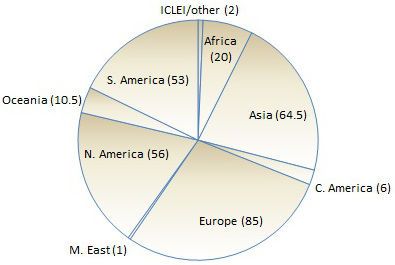
\includegraphics[width=\textwidth]{Fig01.jpg}}
\captionof{figure}{Community gardens in the north of Lisbon (Portugal). \label{Fig01}}
\end{minipage}




\end{multicols}
\vspace{\baselineskip}

\setlength{\tabcolsep}{3pt}
\noindent
\begin{footnotesize}
\begin{minipage}{\columnwidth}\centering
\captionof{table}{Results of a General Linear Model for the proportion of agricultural land under organic farming in French Departments (2008) as a function of plant biodiversity, landscape connectivity, proportion of Natura 2000 protected areas, latitude, longitude, altitude, human population size and department area. The number of data points is 95, the adjusted R$^2$ of the model 0.50, and the intercept 1.457 (s.e. = 2.074).}
\label{Tab01}
\begin{tabular}{lrrrrrrrr}
\toprule
 & N of plant taxa & Landscape connectivity & \% Natura 2000 & Latitude & Longitude & Altitude & Human population & Area \\
\midrule
parameter estimate & 0.264 & 0.047 & 0.113 & -0.084 & 0.003 & 0.038 & 0.056 & 0.327 \\
s.e. & 0.486 & 0.101 & 0.09 & 0.024 & 0.017 & 0.172 & 0.132 & 0.139 \\
\textit{P}-value & 0.59 & 0.64 & 0.21 &\textbf{ \textless0.001} & 0.87 & 0.82 & 0.67 & \textbf{0.02}\\
\bottomrule
\end{tabular}
\end{minipage}

\end{footnotesize}

\vspace{\baselineskip}
\begin{multicols}{2}


\begin{enumerate}[label=\alph*)]
\item
\end{enumerate}